% ---
% title: From Samples to Bits: Sampling Theory and Image Compression
% date: 2026-09-30
% tag: Slides
% excerpt: A 20-minute talk built on one question: how many numbers does an image need? First the sampling theorem (how many samples), then seventy years of image compression read through the spectrum (how many bits per sample, and why the ↓2 and ↑2 inside neural codecs are sampling too), and finally why the two answers are linked: when bits are scarce, fewer samples are better.
% ---
% About 19 minutes: opening 1 min, Part I (how many samples?) 5.5 min,
% Part II (how many bits per sample?) 11 min, Part III (are the two
% answers linked?) 2 min. Each slide answers the question the one before
% it raised; the comment above each frame gives a suggested time.
\documentclass[aspectratio=169]{beamer}
\usetikzlibrary{arrows.meta,positioning,calc,decorations.pathreplacing}
\pgfplotsset{compat=1.18}
\definecolor{sig}{HTML}{1F5FAD}
\definecolor{hot}{HTML}{C0392B}
\definecolor{accent}{HTML}{C77C02}
\definecolor{soft}{HTML}{8C8C8C}
\definecolor{video}{HTML}{2E7D6B}

\title[From Samples to Bits]{From Samples to Bits}
\subtitle{How many numbers does an image need?}
\author{Xu Chen}
\date{October 2026}

\begin{document}

% 0:15
\begin{frame}
  \titlepage
\end{frame}

% 0:50
\begin{frame}{How many numbers does an image need?}
  \begin{center}
  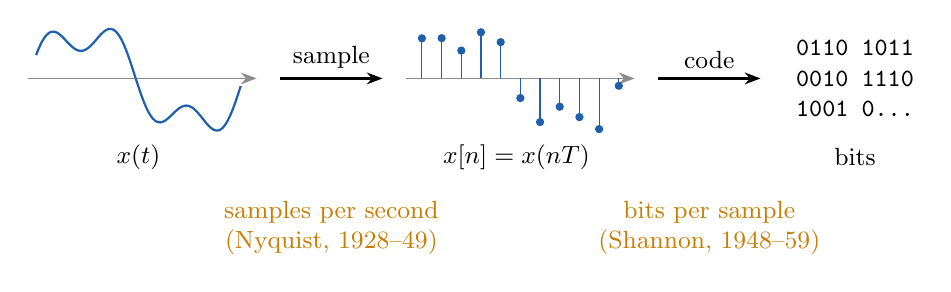
\begin{tikzpicture}[>={Stealth[length=2mm]}, font=\small]
    \draw[soft, ->] (0,0) -- (2.9,0);
    \draw[sig, thick, domain=0.1:2.7, samples=80, smooth] plot (\x, {0.6*sin(130*\x)+0.25*sin(400*\x)});
    \node at (1.4,-1.0) {$x(t)$};
    \draw[->, thick] (3.2,0) -- node[above] {sample} (4.5,0);
    \begin{scope}[xshift=4.8cm]
      \draw[soft, ->] (0,0) -- (2.9,0);
      \foreach \t in {0.2,0.45,...,2.7} {
        \pgfmathsetmacro{\y}{0.6*sin(130*\t)+0.25*sin(400*\t)}
        \draw[sig] (\t,0) -- (\t,\y);
        \fill[sig] (\t,\y) circle (1.5pt);
      }
      \node at (1.4,-1.0) {$x[n]=x(nT)$};
    \end{scope}
    \draw[->, thick] (8.0,0) -- node[above] {code} (9.3,0);
    \node[font=\ttfamily\small, align=left] at (10.5,0) {0110 1011\\0010 1110\\1001 0...};
    \node at (10.5,-1.0) {bits};
    \node[accent, align=center] at (3.85,-1.9) {samples per second\\(Nyquist, 1928--49)};
    \node[accent, align=center] at (8.65,-1.9) {bits per sample\\(Shannon, 1948--59)};
  \end{tikzpicture}
  \end{center}
  \[ \text{bits} \;=\; \text{samples} \times \text{bits per sample} \]
  \begin{enumerate}
    \item \textbf{How many samples?} The sampling theorem.
    \item \textbf{How many bits per sample?} Image compression, from JPEG to learned codecs.
    \item \textbf{Are the two answers independent?} No. One picture explains all three: the \alert{spectrum}.
  \end{enumerate}
\end{frame}

\section{How many samples?}

% 0:40
\begin{frame}{Samples alone are not enough}
  Take a value every $T$ seconds: $x[n]=x(nT)$, at the \textbf{sampling rate} $f_s=1/T$.
  \begin{center}
  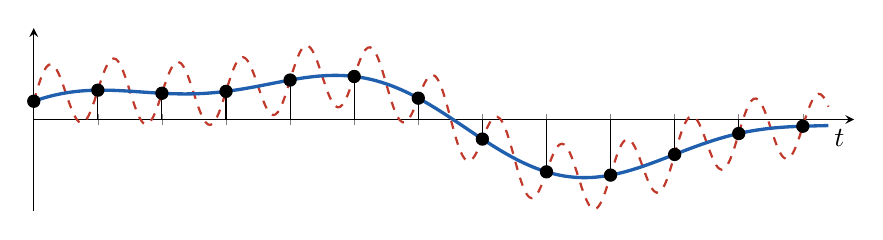
\begin{tikzpicture}
    \begin{axis}[width=12cm, height=3.9cm, axis lines=middle, xmin=0, xmax=6.4, ymin=-2, ymax=2,
        xtick={0,0.5,...,6}, xticklabels={}, ytick=\empty, xlabel={$t$}, clip=false,
        every axis x label/.style={at={(current axis.right of origin)}, anchor=north east}]
      \addplot[hot, thick, dashed, domain=0:6.2, samples=320, smooth]
        {sin(deg(x)) + 0.4*cos(deg(2.3*x)) + 0.7*sin(deg(4*pi*x))};
      \addplot[sig, very thick, domain=0:6.2, samples=150, smooth] {sin(deg(x)) + 0.4*cos(deg(2.3*x))};
      \addplot[black, ycomb, mark=*, mark size=2.2pt, samples at={0,0.5,...,6}] {sin(deg(x)) + 0.4*cos(deg(2.3*x))};
    \end{axis}
  \end{tikzpicture}
  \end{center}
  Both curves pass through the \emph{same} samples. The samples can decide the signal only if it
  \textbf{cannot wiggle too fast} between them, and ``too fast'' is a statement about frequency.
\end{frame}

% 1:00
\begin{frame}{Sampling copies the spectrum}
  \begin{columns}[T]
    \begin{column}{0.5\textwidth}
      \begin{itemize}
        \item $x$ is \textbf{band-limited}: $X(f)=0$ for $|f|>B$.
        \item Sampling multiplies by a Dirac comb:
          \[ x_s(t)=x(t)\sum_n \delta(t-nT) \]
        \item So the spectrum repeats every $f_s$:
          \[ X_s(f)=f_s\sum_k X(f-kf_s) \]
      \end{itemize}
    \end{column}
    \begin{column}{0.5\textwidth}
      \begin{center}
      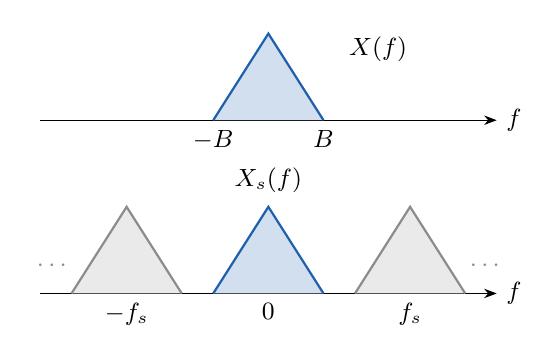
\begin{tikzpicture}[font=\small, >={Stealth[length=1.6mm]}]
        \draw[->] (-2.9,0) -- (2.9,0) node[right] {$f$};
        \filldraw[sig, fill=sig!20, thick] (-0.7,0) -- (0,1.1) -- (0.7,0);
        \node[below] at (-0.7,0) {$-B$};
        \node[below] at (0.7,0) {$B$};
        \node[anchor=west] at (0.9,0.9) {$X(f)$};
        \begin{scope}[yshift=-2.2cm]
          \draw[->] (-2.9,0) -- (2.9,0) node[right] {$f$};
          \foreach \k in {-1,1}
            \filldraw[soft, fill=soft!18, thick] ({1.8*\k-0.7},0) -- ({1.8*\k},1.1) -- ({1.8*\k+0.7},0);
          \filldraw[sig, fill=sig!20, thick] (-0.7,0) -- (0,1.1) -- (0.7,0);
          \node[below] at (-1.8,0) {$-f_s$};
          \node[below] at (0,0) {$0$};
          \node[below] at (1.8,0) {$f_s$};
          \node[soft] at (-2.75,0.35) {$\cdots$};
          \node[soft] at (2.75,0.35) {$\cdots$};
          \node[anchor=south] at (0,1.15) {$X_s(f)$};
        \end{scope}
      \end{tikzpicture}
      \end{center}
      \alert{Sampling in time = copying the spectrum every $f_s$.}
    \end{column}
  \end{columns}
\end{frame}

% 0:45
\begin{frame}{The sampling theorem: the copies must not overlap}
  \begin{block}{Theorem (Nyquist 1928, Shannon 1949 \cite{nyquist1928,shannon1949})}
    If $X(f)=0$ for $|f|>B$ and $f_s>2B$, the samples $x(nT)$ determine $x(t)$ exactly.
  \end{block}
  \begin{center}
  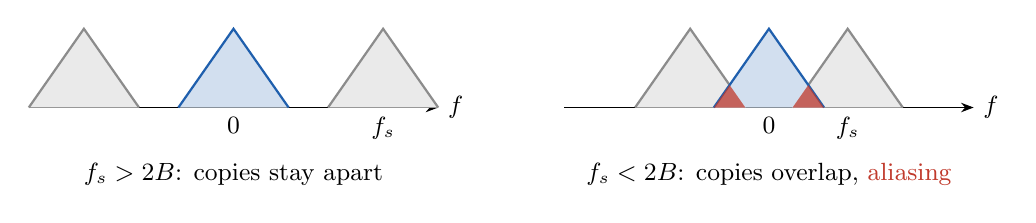
\begin{tikzpicture}[font=\small, >={Stealth[length=1.6mm]}]
    \draw[->] (-2.6,0) -- (2.6,0) node[right] {$f$};
    \foreach \k in {-1,1}
      \filldraw[soft, fill=soft!18, thick] ({1.9*\k-0.7},0) -- ({1.9*\k},1) -- ({1.9*\k+0.7},0);
    \filldraw[sig, fill=sig!20, thick] (-0.7,0) -- (0,1) -- (0.7,0);
    \node[below] at (1.9,0) {$f_s$};
    \node[below] at (0,0) {$0$};
    \node[align=center] at (0,-0.85) {$f_s>2B$: copies stay apart};
    \begin{scope}[xshift=6.8cm]
      \draw[->] (-2.6,0) -- (2.6,0) node[right] {$f$};
      \foreach \k in {-1,1}
        \filldraw[soft, fill=soft!18, thick] ({1.0*\k-0.7},0) -- ({1.0*\k},1) -- ({1.0*\k+0.7},0);
      \filldraw[sig, fill=sig!20, thick] (-0.7,0) -- (0,1) -- (0.7,0);
      \fill[hot, opacity=0.75] (0.3,0) -- (0.5,0.2857) -- (0.7,0) -- cycle;
      \fill[hot, opacity=0.75] (-0.3,0) -- (-0.5,0.2857) -- (-0.7,0) -- cycle;
      \node[below] at (1.0,0) {$f_s$};
      \node[below] at (0,0) {$0$};
      \node[align=center] at (0,-0.85) {$f_s<2B$: copies overlap, \textcolor{hot}{aliasing}};
    \end{scope}
  \end{tikzpicture}
  \end{center}
  $2B$ is the \textbf{Nyquist rate}. Two cases follow: how to get $x$ back, and what goes wrong below it.
\end{frame}

% 1:05
\begin{frame}{Inside the band: a sinc puts the signal back}
  \begin{columns}[T]
    \begin{column}{0.44\textwidth}
      \begin{itemize}
        \item Keep the central copy with an ideal \textbf{low-pass} at $f_s/2$.
        \item In time, that filter is a sinc: $\operatorname{sinc}(u)=\frac{\sin\pi u}{\pi u}$. Each sample adds one.
        \item In practice short kernels approximate it: linear, cubic, Lanczos.
        \item Remember the sinc's \alert{ripples}: they come back in JPEG.
      \end{itemize}
    \end{column}
    \begin{column}{0.56\textwidth}
      \begin{center}
      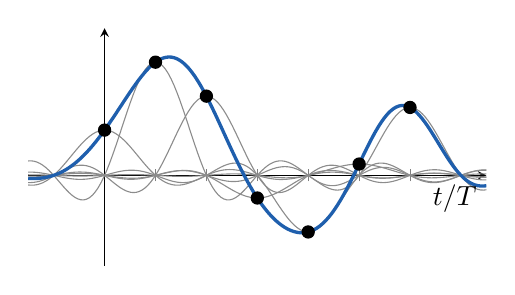
\begin{tikzpicture}[declare function={s(\t)=sin(180*\t)/(pi*\t);}]
        \begin{axis}[width=7.4cm, height=4.6cm, axis lines=middle, xmin=-1.5, xmax=7.5, ymin=-0.8, ymax=1.3,
            xtick={0,...,6}, xticklabels={}, ytick=\empty, xlabel={$t/T$},
            every axis x label/.style={at={(current axis.right of origin)}, anchor=north east},
            domain=-1.5:7.5, samples=158, no markers]
          \addplot[soft] {0.4*s(x)};
          \addplot[soft] {1.0*s(x-1)};
          \addplot[soft] {0.7*s(x-2)};
          \addplot[soft] {-0.2*s(x-3)};
          \addplot[soft] {-0.5*s(x-4)};
          \addplot[soft] {0.1*s(x-5)};
          \addplot[soft] {0.6*s(x-6)};
          \addplot[sig, very thick] {0.4*s(x)+1.0*s(x-1)+0.7*s(x-2)-0.2*s(x-3)-0.5*s(x-4)+0.1*s(x-5)+0.6*s(x-6)};
          \addplot[black, only marks, mark=*, mark size=2.2pt]
            coordinates {(0,0.4) (1,1.0) (2,0.7) (3,-0.2) (4,-0.5) (5,0.1) (6,0.6)};
        \end{axis}
      \end{tikzpicture}
      \end{center}
    \end{column}
  \end{columns}
  \[ x(t)=\sum_{n} x[n]\,\operatorname{sinc}\Big(\frac{t-nT}{T}\Big) \]
\end{frame}

% 0:45
\begin{frame}{Outside the band: aliasing, unless we blur first}
  \begin{center}
  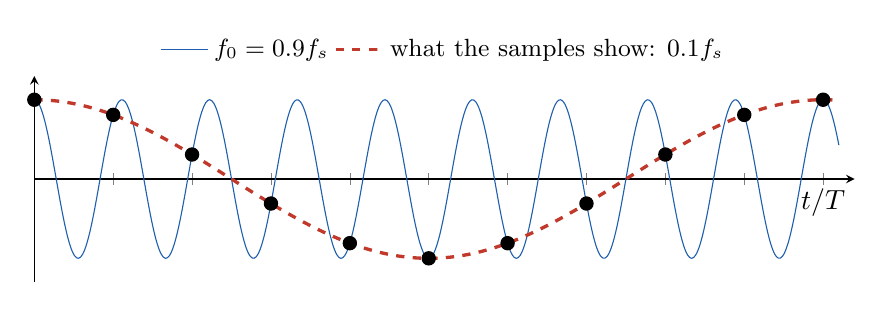
\begin{tikzpicture}
    \begin{axis}[width=12cm, height=4.2cm, axis lines=middle, xmin=0, xmax=10.4, ymin=-1.3, ymax=1.3,
        xtick={0,...,10}, xticklabels={}, ytick=\empty, xlabel={$t/T$}, clip=false,
        every axis x label/.style={at={(current axis.right of origin)}, anchor=north east},
        legend style={draw=none, fill=none, font=\small, at={(0.5,1.02)}, anchor=south, legend columns=2}]
      \addplot[sig, domain=0:10.2, samples=400, smooth] {cos(deg(2*pi*0.9*x))};
      \addlegendentry{$f_0=0.9f_s$}
      \addplot[hot, very thick, dashed, domain=0:10.2, samples=120, smooth] {cos(deg(2*pi*0.1*x))};
      \addlegendentry{what the samples show: $0.1f_s$}
      \addplot[black, only marks, mark=*, mark size=2.4pt, samples at={0,...,10}] {cos(deg(2*pi*0.1*x))};
    \end{axis}
  \end{tikzpicture}
  \end{center}
  \begin{itemize}
    \item The samples cannot tell $f_0$ from $|f_0-f_s|$: a fast wave poses as a slow one. Moir\'e, jaggies, wheels turning backwards.
    \item \alert{It cannot be undone} after sampling. The only cure is a \textbf{low-pass before sampling}.
  \end{itemize}
\end{frame}

% 1:05
\begin{frame}{Images: a low-pass around every resize}
  \begin{columns}[T]
    \begin{column}{0.56\textwidth}
      \begin{itemize}
        \item A pixel grid samples the scene in 2-D: frequencies up to $\tfrac12$ cycle per pixel.
        \item \textbf{Shrink} ($\downarrow2$): the limit drops to $\tfrac14$. Blur first, or the \textcolor{hot}{red} part aliases. Image pyramids do exactly this \cite{burt1983}.
        \item \textbf{Enlarge} ($\uparrow2$): insert zeros, then interpolate, which is the same low-pass.
        \item So the pixel count is fixed by the finest detail kept: 12 megapixels, 36\,MB raw.
          \alert{How few bits can each pixel get?}
      \end{itemize}
    \end{column}
    \begin{column}{0.44\textwidth}
      \begin{center}
      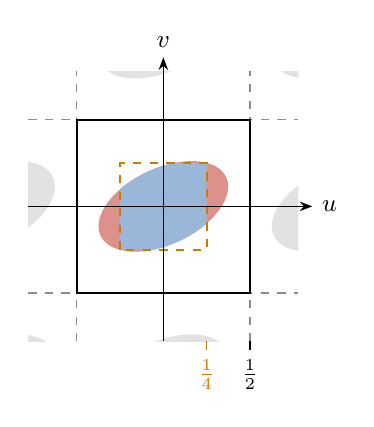
\begin{tikzpicture}[scale=2.2, font=\small, >={Stealth[length=1.6mm]}]
        \begin{scope}
          \clip (-0.78,-0.78) rectangle (0.78,0.78);
          \foreach \a/\b in {-1/0,1/0,0/-1,0/1,-1/-1,-1/1,1/-1,1/1}
            \fill[soft!25, rotate around={25:(\a,\b)}] (\a,\b) ellipse (0.4 and 0.22);
          \draw[soft, dashed] (-0.78,-0.5) -- (0.78,-0.5) (-0.78,0.5) -- (0.78,0.5)
            (-0.5,-0.78) -- (-0.5,0.78) (0.5,-0.78) -- (0.5,0.78);
        \end{scope}
        \fill[hot!55, rotate=25] (0,0) ellipse (0.4 and 0.22);
        \begin{scope}
          \clip (-0.25,-0.25) rectangle (0.25,0.25);
          \fill[sig!45, rotate=25] (0,0) ellipse (0.4 and 0.22);
        \end{scope}
        \draw[thick] (-0.5,-0.5) rectangle (0.5,0.5);
        \draw[accent, thick, dashed] (-0.25,-0.25) rectangle (0.25,0.25);
        \draw[->] (-0.78,0) -- (0.86,0) node[right] {$u$};
        \draw[->] (0,-0.78) -- (0,0.86) node[above] {$v$};
        \draw (0.5,-0.78) -- ++(0,-0.05) node[below] {$\frac12$};
        \draw[accent] (0.25,-0.78) -- ++(0,-0.05) node[below] {$\frac14$};
      \end{tikzpicture}
      \end{center}
      {\small Grey: copies. Dashed: limit after $\downarrow2$.}
    \end{column}
  \end{columns}
\end{frame}

\section{How many bits per sample?}

% 0:55
\begin{frame}{Images compress because their spectrum falls fast}
  \begin{center}
  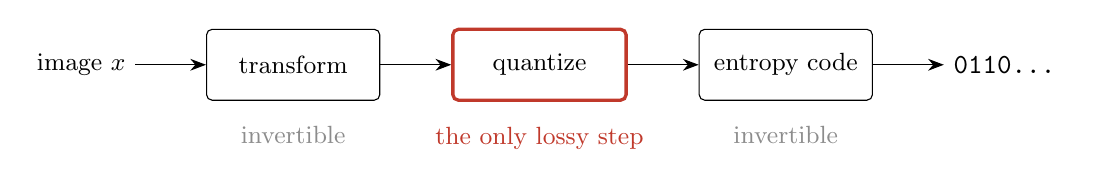
\begin{tikzpicture}[font=\small, >={Stealth[length=2mm]}, node distance=9mm,
      box/.style={draw, rounded corners=2pt, minimum height=9mm, minimum width=22mm, align=center}]
    \node (x) {image $x$};
    \node[box, right=of x] (t) {transform};
    \node[box, right=of t, draw=hot, very thick] (q) {quantize};
    \node[box, right=of q] (e) {entropy code};
    \node[right=of e, font=\ttfamily] (b) {0110...};
    \draw[->] (x) -- (t);
    \draw[->] (t) -- (q);
    \draw[->] (q) -- (e);
    \draw[->] (e) -- (b);
    \node[below=2mm of t, soft] {invertible};
    \node[below=2mm of q, hot] {the only lossy step};
    \node[below=2mm of e, soft] {invertible};
  \end{tikzpicture}
  \end{center}
  \begin{itemize}
    \item \textbf{Redundancy}: neighbouring pixels are alike, so the spectrum of natural images falls like $1/f^2$ \cite{field1987}. Most energy sits in a few low frequencies.
    \item \textbf{Irrelevance}: the eye barely sees fine detail, and fine colour even less.
    \item Every codec: \textbf{transform} to find the frequencies, \textbf{quantize}, \textbf{entropy-code}.
      \alert{How few bits are possible?}
  \end{itemize}
\end{frame}

% 1:05
\begin{frame}{The limit: spend bits only above the water level}
  \begin{columns}[T]
    \begin{column}{0.46\textwidth}
      \textbf{Rate--distortion} \cite{shannon1959}: the fewest bits for a given error.
      For a spectrum, the answer is \textbf{reverse water-filling} \cite{berger1971}:
      \begin{itemize}
        \item Frequencies above the level $\theta$ get bits; those below get \alert{none}.
        \item Fewer bits $\Rightarrow$ higher $\theta$ $\Rightarrow$ narrower band.
        \item The ideal lossy code is a \textbf{low-pass set by the budget}.
      \end{itemize}
    \end{column}
    \begin{column}{0.54\textwidth}
      \begin{center}
      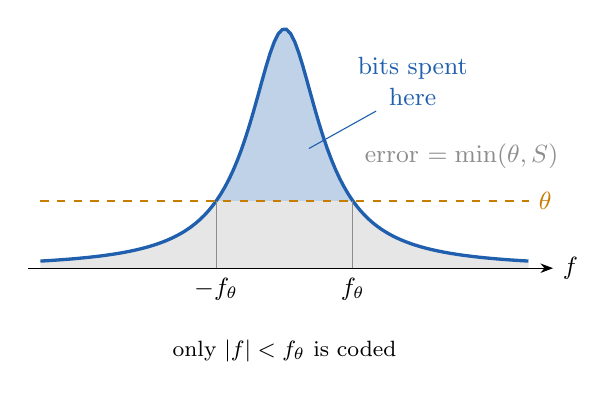
\begin{tikzpicture}[x=1.55cm, y=1.9cm, font=\small, >={Stealth[length=1.6mm]},
          declare function={S(\t)=1.6/(1+(\t/0.35)^2);}]
        \fill[soft!22] (-2,0) -- plot[domain=-2:-0.56, samples=50] (\x,{S(\x)}) -- (0.56,0.45)
          -- plot[domain=0.56:2, samples=50] (\x,{S(\x)}) -- (2,0) -- cycle;
        \fill[sig!28] (-0.56,0.45) -- plot[domain=-0.56:0.56, samples=60] (\x,{S(\x)}) -- cycle;
        \draw[sig, very thick] plot[domain=-2:2, samples=120] (\x,{S(\x)});
        \draw[accent, thick, dashed] (-2,0.45) -- (2,0.45) node[right] {$\theta$};
        \draw[->] (-2.1,0) -- (2.2,0) node[right] {$f$};
        \draw[soft] (-0.56,0) -- (-0.56,0.45);
        \draw[soft] (0.56,0) -- (0.56,0.45);
        \node[below] at (-0.56,0) {$-f_\theta$};
        \node[below] at (0.56,0) {$f_\theta$};
        \node[sig, align=center] at (1.05,1.25) {bits spent\\here};
        \draw[sig] (0.75,1.05) -- (0.2,0.8);
        \node[soft, align=center] at (1.45,0.75) {error $=\min(\theta,S)$};
        \node[align=center, font=\footnotesize] at (0,-0.55) {only $|f|<f_\theta$ is coded};
      \end{tikzpicture}
      \end{center}
    \end{column}
  \end{columns}
  \medskip
  Theory says \emph{what} to keep, not \emph{how}. Seventy years of codecs approximate this picture.
\end{frame}

% 0:40
\begin{frame}{Seventy years of codecs, each fixing the last}
  \begin{center}
  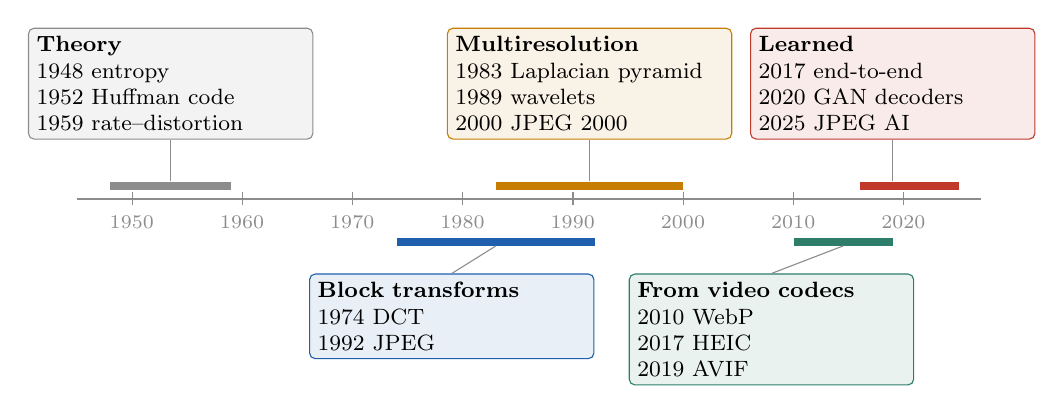
\begin{tikzpicture}[font=\footnotesize, x=0.14cm,
      era/.style={draw=#1, fill=#1!10, rounded corners=2pt, align=left, inner sep=3pt, text width=3.4cm},
      span/.style={#1, line width=3pt}]
    \draw[soft, thick] (1945,0) -- (2027,0);
    \foreach \y in {1950,1960,...,2020} {
      \draw[soft] (\y,-0.08) -- (\y,0.08);
      \node[soft, font=\scriptsize] at (\y,-0.3) {\y};
    }
    \draw[span=soft] (1948,0.16) -- (1959,0.16);
    \draw[span=sig] (1974,-0.55) -- (1992,-0.55);
    \draw[span=accent] (1983,0.16) -- (2000,0.16);
    \draw[span=video] (2010,-0.55) -- (2019,-0.55);
    \draw[span=hot] (2016,0.16) -- (2025,0.16);
    \node[era=soft, anchor=south] (a) at (1953.5,0.75) {\textbf{Theory}\\1948 entropy\\1952 Huffman code\\1959 rate--distortion};
    \node[era=accent, anchor=south] (c) at (1991.5,0.75) {\textbf{Multiresolution}\\1983 Laplacian pyramid\\1989 wavelets\\2000 JPEG 2000};
    \node[era=hot, anchor=south] (e) at (2019,0.75) {\textbf{Learned}\\2017 end-to-end\\2020 GAN decoders\\2025 JPEG AI};
    \node[era=sig, anchor=north] (b) at (1979,-0.95) {\textbf{Block transforms}\\1974 DCT\\1992 JPEG};
    \node[era=video, anchor=north] (d) at (2008,-0.95) {\textbf{From video codecs}\\2010 WebP\\2017 HEIC\\2019 AVIF};
    \draw[soft] (a.south) -- (1953.5,0.22);
    \draw[soft] (c.south) -- (1991.5,0.22);
    \draw[soft] (e.south) -- (2019,0.22);
    \draw[soft] (b.north) -- (1983,-0.6);
    \draw[soft] (d.north) -- (2014.5,-0.6);
  \end{tikzpicture}
  \end{center}
  JPEG's blocks $\to$ whole-image wavelets $\to$ prediction $\to$ learned transforms $\to$ generated detail.
\end{frame}

% 0:45
\begin{frame}{JPEG (1992): less colour, then frequencies}
  \begin{center}
  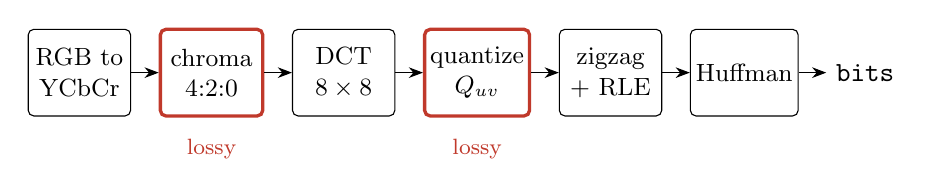
\begin{tikzpicture}[font=\small, >={Stealth[length=1.8mm]}, node distance=3.5mm,
      box/.style={draw, rounded corners=2pt, minimum height=11mm, minimum width=13mm, align=center, inner sep=2pt}]
    \node[box] (c) {RGB to\\YCbCr};
    \node[box, right=of c, draw=hot, very thick] (s) {chroma\\4:2:0};
    \node[box, right=of s] (d) {DCT\\$8\times8$};
    \node[box, right=of d, draw=hot, very thick] (q) {quantize\\$Q_{uv}$};
    \node[box, right=of q] (z) {zigzag\\+ RLE};
    \node[box, right=of z] (h) {Huffman};
    \node[right=of h, font=\ttfamily] (b) {bits};
    \draw[->] (c) -- (s);
    \draw[->] (s) -- (d);
    \draw[->] (d) -- (q);
    \draw[->] (q) -- (z);
    \draw[->] (z) -- (h);
    \draw[->] (h) -- (b);
    \node[below=1.5mm of s, hot, font=\footnotesize] {lossy};
    \node[below=1.5mm of q, hot, font=\footnotesize] {lossy};
  \end{tikzpicture}
  \end{center}
  \begin{itemize}
    \item \textbf{Chroma 4:2:0}: the eye sees colour at low resolution, so colour is blurred and
      \textbf{downsampled by 2} each way. Part I's rule, used on purpose: half the samples, gone.
    \item \textbf{$8\times8$ DCT}: each block written as frequencies \cite{ahmed1974}.
    \item Then quantize, and entropy-code the result \cite{wallace1992}. The bits are saved in the quantizer.
  \end{itemize}
\end{frame}

% 0:50
\begin{frame}{JPEG: the quantization table is a water level}
  \begin{columns}[T]
    \begin{column}{0.56\textwidth}
      \begin{itemize}
        \item Neighbouring pixels are alike, so a block's energy piles into the few top-left (low-frequency) coefficients.
        \item Quantize: $\hat c_{uv}=Q_{uv}\,\mathrm{round}(c_{uv}/Q_{uv})$. The step is about 16 at the top left and about 100 at the bottom right.
        \item Anything below half a step becomes $0$ and costs almost nothing.
        \item \alert{Water-filling by hand}, block by block: a low-pass on each block.
      \end{itemize}
    \end{column}
    \begin{column}{0.44\textwidth}
      \begin{center}
      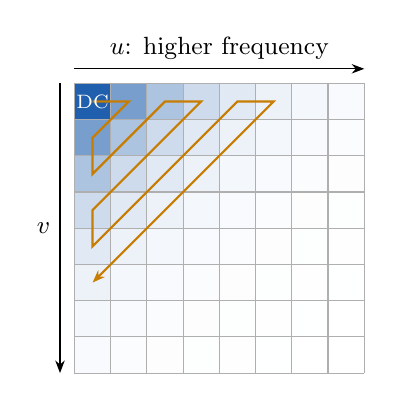
\begin{tikzpicture}[scale=0.46, font=\small, >={Stealth[length=1.6mm]}]
        \foreach \i in {0,...,7} \foreach \j in {0,...,7} {
          \pgfmathsetmacro{\o}{100*exp(-0.5*(\i+\j))}
          \fill[sig!\o!white] (\i,-\j) rectangle ++(1,-1);
        }
        \draw[step=1, soft!70] (0,0) grid (8,-8);
        \draw[accent, thick, ->] (0.5,-0.5) -- (1.5,-0.5) -- (0.5,-1.5) -- (0.5,-2.5) -- (1.5,-1.5) -- (2.5,-0.5) -- (3.5,-0.5) -- (2.5,-1.5) -- (1.5,-2.5) -- (0.5,-3.5) -- (0.5,-4.5) -- (1.5,-3.5) -- (2.5,-2.5) -- (3.5,-1.5) -- (4.5,-0.5) -- (5.5,-0.5) -- (4.5,-1.5) -- (3.5,-2.5) -- (2.5,-3.5) -- (1.5,-4.5) -- (0.5,-5.5);
        \node[white, font=\scriptsize] at (0.5,-0.5) {DC};
        \draw[->] (0,0.4) -- node[above] {$u$: higher frequency} (8,0.4);
        \draw[->] (-0.4,0) -- node[left] {$v$} (-0.4,-8);
      \end{tikzpicture}
      \end{center}
      {\small Typical $|c_{uv}|$, and the zigzag scan.}
    \end{column}
  \end{columns}
\end{frame}

% 0:50
\begin{frame}{JPEG's flaws: blocks, and the sinc again}
  \begin{columns}[T]
    \begin{column}{0.5\textwidth}
      \begin{itemize}
        \item \textbf{Blocking}: blocks are coded independently; at low rates their borders no longer match.
        \item \textbf{Ringing}: cutting a block's high frequencies is an ideal low-pass, i.e.\ a convolution with the \alert{sinc} of Part I. Its ripples appear beside every edge.
        \item This is low-pass filtering, \emph{not} downsampling: the pixel count is unchanged.
      \end{itemize}
    \end{column}
    \begin{column}{0.5\textwidth}
      \begin{center}
      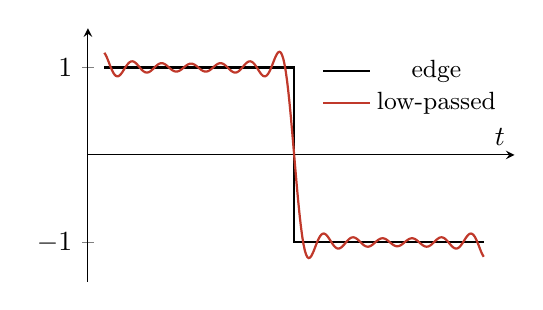
\begin{tikzpicture}
        \begin{axis}[width=7cm, height=4.8cm, axis lines=middle, xmin=0, xmax=6.5, ymin=-1.45, ymax=1.45,
            xtick=\empty, ytick={-1,1}, xlabel={$t$}, no markers,
            legend style={draw=none, fill=none, font=\small, at={(0.99,0.92)}, anchor=north east}]
          \addplot[black, thick, const plot] coordinates {(0.25,1) (3.1416,-1) (6.03,-1)};
          \addlegendentry{edge}
          \addplot[hot, thick, domain=0.25:6.03, samples=300]
            {4/pi*(sin(deg(x)) + sin(deg(3*x))/3 + sin(deg(5*x))/5 + sin(deg(7*x))/7 + sin(deg(9*x))/9 + sin(deg(11*x))/11 + sin(deg(13*x))/13)};
          \addlegendentry{low-passed}
        \end{axis}
      \end{tikzpicture}
      \end{center}
    \end{column}
  \end{columns}
  \medskip
  To lose the blocks: transform the \emph{whole} image, at every scale.
\end{frame}

% 1:10
\begin{frame}{Wavelets (JPEG 2000): aliasing that cancels}
  \begin{columns}[T]
    \begin{column}{0.64\textwidth}
      \begin{center}
      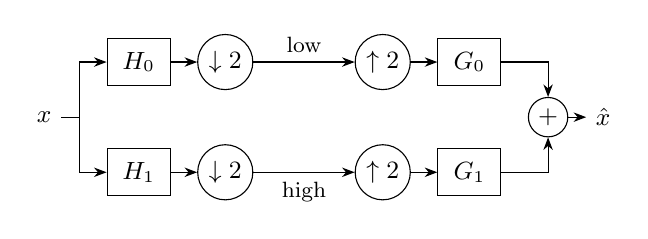
\begin{tikzpicture}[font=\small, >={Stealth[length=1.6mm]},
          f/.style={draw, minimum width=8mm, minimum height=6mm, inner sep=1pt},
          r/.style={draw, circle, inner sep=0pt, minimum size=7mm}]
        \node (x) at (0,0) {$x$};
        \node[f] (h0) at (1.2,0.7) {$H_0$};
        \node[f] (h1) at (1.2,-0.7) {$H_1$};
        \node[r] (d0) at (2.3,0.7) {$\downarrow 2$};
        \node[r] (d1) at (2.3,-0.7) {$\downarrow 2$};
        \node[r] (u0) at (4.3,0.7) {$\uparrow 2$};
        \node[r] (u1) at (4.3,-0.7) {$\uparrow 2$};
        \node[f] (g0) at (5.4,0.7) {$G_0$};
        \node[f] (g1) at (5.4,-0.7) {$G_1$};
        \node[draw, circle, inner sep=0pt, minimum size=5mm] (s) at (6.4,0) {$+$};
        \node (y) at (7.1,0) {$\hat x$};
        \draw[->] (x) -- (0.45,0) |- (h0);
        \draw[->] (0.45,0) |- (h1);
        \draw[->] (h0) -- (d0);
        \draw[->] (h1) -- (d1);
        \draw[->] (d0) -- node[above, font=\footnotesize] {low} (u0);
        \draw[->] (d1) -- node[below, font=\footnotesize] {high} (u1);
        \draw[->] (u0) -- (g0);
        \draw[->] (u1) -- (g1);
        \draw[->] (g0) -| (s);
        \draw[->] (g1) -| (s);
        \draw[->] (s) -- (y);
      \end{tikzpicture}
      \end{center}
    \end{column}
    \begin{column}{0.36\textwidth}
      \begin{center}
      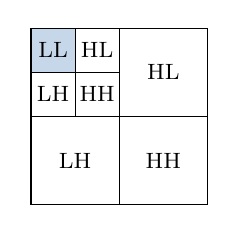
\begin{tikzpicture}[font=\footnotesize, scale=0.8]
        \fill[sig!25] (0,2.1) rectangle (0.7,2.8);
        \draw (0,0) rectangle (2.8,2.8);
        \draw (1.4,0) -- (1.4,2.8);
        \draw (0,1.4) -- (2.8,1.4);
        \draw (0.7,1.4) -- (0.7,2.8);
        \draw (0,2.1) -- (1.4,2.1);
        \node at (0.35,2.45) {LL};
        \node at (1.05,2.45) {HL};
        \node at (0.35,1.75) {LH};
        \node at (1.05,1.75) {HH};
        \node at (2.1,2.1) {HL};
        \node at (0.7,0.7) {LH};
        \node at (2.1,0.7) {HH};
      \end{tikzpicture}
      \end{center}
    \end{column}
  \end{columns}
  \begin{itemize}
    \item Split into low and high half-bands, \textbf{downsample each by 2}; repeat on the low band \cite{mallat1989}.
    \item Each $\downarrow2$ aliases, but $G_0,G_1$ are designed so the two aliases \alert{cancel exactly}. No blocks, every resolution in one bitstream \cite{skodras2001}.
    \item Another road, taken by video codecs: do not transform everything, \alert{predict}.
  \end{itemize}
\end{frame}

% 1:10
\begin{frame}{Prediction: code only the surprise}
  \begin{columns}[T]
    \begin{column}{0.5\textwidth}
      \begin{center}
      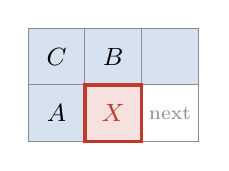
\begin{tikzpicture}[font=\small, scale=0.72]
        \fill[sig!18] (0,0) rectangle (3,1);
        \fill[sig!18] (0,0) rectangle (1,-1);
        \fill[hot!15] (1,0) rectangle (2,-1);
        \draw[soft, step=1] (0,-1) grid (3,1);
        \draw[hot, very thick] (1,0) rectangle (2,-1);
        \node at (0.5,0.5) {$C$};
        \node at (1.5,0.5) {$B$};
        \node at (0.5,-0.5) {$A$};
        \node[hot] at (1.5,-0.5) {$X$};
        \node[soft, font=\scriptsize] at (2.5,-0.5) {next};
      \end{tikzpicture}
      \end{center}
      \textbf{PNG} (1996), lossless \cite{boutell1997}
      \begin{itemize}
        \item Guess each pixel from its left and upper neighbours; keep only the error, mostly near $0$.
        \item DEFLATE (LZ77 + Huffman) packs the errors. No quantizer: nothing is lost.
        \item Small for screenshots, large for photos.
      \end{itemize}
    \end{column}
    \begin{column}{0.5\textwidth}
      \begin{center}
      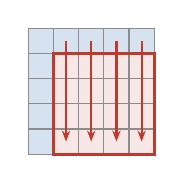
\begin{tikzpicture}[font=\small, scale=0.8, >={Stealth[length=1.4mm]}]
        \fill[sig!18] (-0.4,0.4) rectangle (1.6,0.8);
        \fill[sig!18] (-0.4,-1.2) rectangle (0,0.4);
        \fill[hot!12] (0,-1.2) rectangle (1.6,0.4);
        \draw[soft, step=0.4] (-0.4,-1.2) grid (1.6,0.8);
        \draw[hot, very thick] (0,-1.2) rectangle (1.6,0.4);
        \foreach \x in {0.2,0.6,1.0,1.4} \draw[->, hot, thick] (\x,0.6) -- (\x,-1.0);
      \end{tikzpicture}
      \end{center}
      \textbf{WebP} (2010), lossy \cite{bankoski2011,zern2024}
      \begin{itemize}
        \item From the VP8 video codec: guess a whole block from the decoded pixels above and to its left.
        \item DCT and quantize only the error: JPEG on the surprise; a deblocking filter smooths block edges.
        \item HEIC and AVIF push the same idea further.
      \end{itemize}
    \end{column}
  \end{columns}
\end{frame}

% 1:00
\begin{frame}{Learned codecs (2017--): learn the whole pipeline}
  \begin{center}
  \begin{tikzpicture}[nn, node distance=4mm, nndata/.append style={minimum width=8mm}]
    \node[nndata] (x) {$x$};
    \node[nnenc, right=of x] (ga) {$g_a$\\conv $\downarrow2$\\$\times4$};
    \node[nnfeat, right=of ga] (y) {$y$};
    \node[nnbox={nnactc}{9mm}, right=of y] (q) {$Q$};
    \node[nnbox={nnfcc}{10mm}, right=of q] (ae) {AE};
    \node[right=of ae, font=\ttfamily\small] (bits) {bits};
    \node[nnbox={nnfcc}{10mm}, right=of bits] (ad) {AD};
    \node[nndec, right=of ad] (gs) {$g_s$\\deconv $\uparrow2$\\$\times4$};
    \node[nndata, right=of gs] (xh) {$\hat x$};
    \node[nnbox={nnnormc}{20mm}, above=6mm of bits] (p) {entropy model $p(\hat y)$};
    \draw[nnflow] (x) -- (ga);
    \draw[nnflow] (ga) -- (y);
    \draw[nnflow] (y) -- (q);
    \draw[nnflow] (q) -- (ae);
    \draw[nnflow] (ae) -- (bits);
    \draw[nnflow] (bits) -- (ad);
    \draw[nnflow] (ad) -- (gs);
    \draw[nnflow] (gs) -- (xh);
    \draw[nnflow, dashed] (p) -| (ae);
    \draw[nnflow, dashed] (p) -| (ad);
  \end{tikzpicture}
  \end{center}
  \[ \mathcal L = R + \lambda D = \mathbb E\big[-\log_2 p(\hat y)\big] + \lambda\,\mathbb E\big[\|x-\hat x\|^2\big] \]
  \begin{itemize}
    \item The same three steps as JPEG, every one learned, trained on bits plus error \cite{balle2017,balle2018}:
      water-filling learned from data. On par with VVC by 2020 \cite{cheng2020}; a standard, JPEG AI, in 2025 \cite{jpegai2025}.
    \item Its $\downarrow2$ and $\uparrow2$: an engineering habit, or \alert{sampling theory}?
  \end{itemize}
\end{frame}

% 1:20
\begin{frame}{$\uparrow2$ and $\downarrow2$ in networks are sampling too}
  \begin{columns}[T]
    \begin{column}{0.56\textwidth}
      \begin{itemize}
        \item \textbf{$\uparrow2$} inserts zeros, which adds a \textcolor{hot}{copy} of the spectrum at $\tfrac12$. The next conv must remove it: it \emph{is} an interpolation filter.
        \item A copy left in is a \textbf{checkerboard} (e.g.\ transposed conv, kernel 3, stride 2) \cite{odena2016}. Fix: resize then conv, or sub-pixel conv with ICNR \cite{shi2016,aitken2017}.
        \item \textbf{$\downarrow2$} without a blur aliases: a one-pixel shift changes the output \cite{zhang2019,karras2021}.
      \end{itemize}
    \end{column}
    \begin{column}{0.44\textwidth}
      \begin{center}
      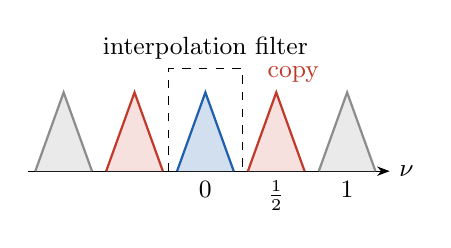
\begin{tikzpicture}[x=1.8cm, font=\small, >={Stealth[length=1.6mm]}]
        \draw[->] (-1.25,0) -- (1.3,0) node[right] {$\nu$};
        \foreach \c in {-1,1}
          \filldraw[soft, fill=soft!18, thick] ({\c-0.2},0) -- (\c,1) -- ({\c+0.2},0);
        \foreach \c in {-0.5,0.5}
          \filldraw[hot, fill=hot!15, thick] ({\c-0.2},0) -- (\c,1) -- ({\c+0.2},0);
        \filldraw[sig, fill=sig!20, thick] (-0.2,0) -- (0,1) -- (0.2,0);
        \draw[black, dashed] (-0.26,0) -- (-0.26,1.3) -- (0.26,1.3) -- (0.26,0);
        \node[above] at (0,1.3) {interpolation filter};
        \node[hot, above] at (0.62,1) {copy};
        \node[below] at (0,0) {$0$};
        \node[below] at (0.5,0) {$\frac{1}{2}$};
        \node[below] at (1,0) {$1$};
      \end{tikzpicture}
      \end{center}
      {\small After inserting zeros.}
    \end{column}
  \end{columns}
  \medskip
  Practical, \emph{and} the sampling theorem says why it works and when it fails.
\end{frame}

% 1:05
\begin{frame}{What happens to the frequencies we dropped?}
  \begin{columns}[T]
    \begin{column}{0.5\textwidth}
      \begin{itemize}
        \item At low rates nothing above $f_\theta$ is sent.
        \item An \textbf{MSE-optimal} decoder fills in the average, zero: \textbf{blurry}.
        \item A \textbf{generative} decoder fills in plausible detail \cite{mentzer2020,yang2023}: sharp, but \alert{generated, not transmitted}.
        \item Error and realism trade off \cite{blau2018,blau2019}.
      \end{itemize}
    \end{column}
    \begin{column}{0.5\textwidth}
      \begin{center}
      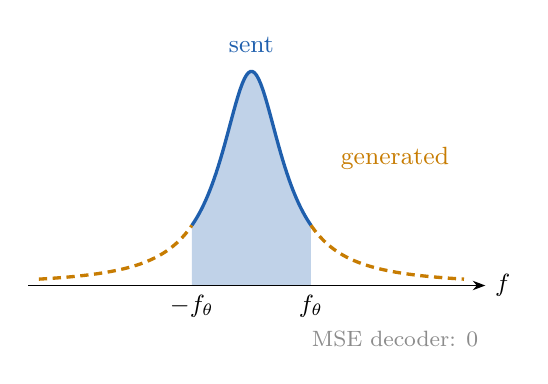
\begin{tikzpicture}[x=1.35cm, y=1.7cm, font=\small, >={Stealth[length=1.6mm]},
          declare function={S(\t)=1.6/(1+(\t/0.35)^2);}]
        \fill[sig!28] (-0.56,0) -- plot[domain=-0.56:0.56, samples=60] (\x,{S(\x)}) -- (0.56,0) -- cycle;
        \draw[sig, very thick] plot[domain=-0.56:0.56, samples=60] (\x,{S(\x)});
        \draw[accent, very thick, densely dashed] plot[domain=0.56:2, samples=50] (\x,{S(\x)});
        \draw[accent, very thick, densely dashed] plot[domain=-2:-0.56, samples=50] (\x,{S(\x)});
        \draw[->] (-2.1,0) -- (2.2,0) node[right] {$f$};
        \node[below] at (-0.56,0) {$-f_\theta$};
        \node[below] at (0.56,0) {$f_\theta$};
        \node[sig] at (0,1.8) {sent};
        \node[accent, align=center] at (1.35,0.95) {generated};
        \node[soft, align=center, font=\footnotesize] at (1.35,-0.4) {MSE decoder: $0$};
      \end{tikzpicture}
      \end{center}
    \end{column}
  \end{columns}
  \medskip
  So far the pixel count was fixed. If a codec drops everything above $f_\theta$, \alert{why sample it at all?}
\end{frame}

\section{Are the two answers linked?}

% 1:05
\begin{frame}{When bits are scarce, sample less}
  \begin{columns}[T]
    \begin{column}{0.54\textwidth}
      \begin{itemize}
        \item \textbf{Theory}: at bitrate $R$, sampling at $2f_\theta$, below Nyquist, already reaches the best error $D(R)$ \cite{kipnis2016,kipnis2018}.
        \item \textbf{Images}: downscale, JPEG, upscale beats plain JPEG at low rates \cite{bruckstein2003}.
        \item \textbf{Practice}: AV1 codes frames narrower and upscales them in the loop \cite{av1overview}; streaming picks a resolution for each bitrate \cite{netflix2015}.
        \item Part I's rule still holds: blur before shrinking. At low rates that blur is free.
      \end{itemize}
    \end{column}
    \begin{column}{0.46\textwidth}
      \begin{center}
      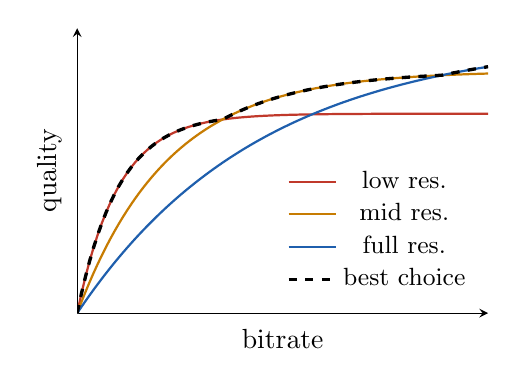
\begin{tikzpicture}
        \begin{axis}[width=6.8cm, height=5.2cm, axis lines=left, xmin=0, xmax=10, ymin=0, ymax=100,
            xlabel={bitrate}, ylabel={quality}, xtick=\empty, ytick=\empty, no markers, samples=100, domain=0:10,
            legend style={draw=none, fill=none, font=\small, at={(0.98,0.04)}, anchor=south east}]
          \addplot[hot, thick] {70*(1-exp(-x/1.0))};
          \addlegendentry{low res.}
          \addplot[accent, thick] {85*(1-exp(-x/2.2))};
          \addlegendentry{mid res.}
          \addplot[sig, thick] {97*(1-exp(-x/4.5))};
          \addlegendentry{full res.}
          \addplot[black, very thick, dashed] {max(70*(1-exp(-x/1.0)), 85*(1-exp(-x/2.2)), 97*(1-exp(-x/4.5)))};
          \addlegendentry{best choice}
        \end{axis}
      \end{tikzpicture}
      \end{center}
      {\small Schematic.}
    \end{column}
  \end{columns}
\end{frame}

% 0:45
\begin{frame}{One picture for the whole talk}
  \begin{center}
  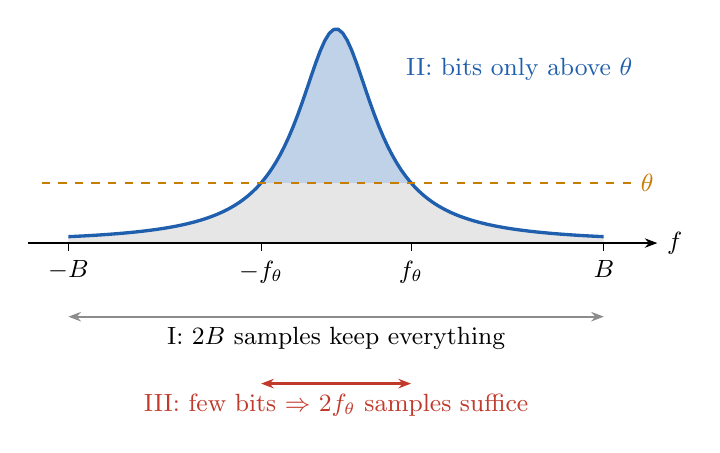
\begin{tikzpicture}[x=1.7cm, y=1.7cm, font=\small, >={Stealth[length=1.6mm]},
      declare function={S(\t)=1.6/(1+(\t/0.35)^2);}]
    \fill[soft!22] (-2,0) -- plot[domain=-2:2, samples=120] (\x,{S(\x)}) -- (2,0) -- cycle;
    \fill[sig!28] (-0.56,0.45) -- plot[domain=-0.56:0.56, samples=60] (\x,{S(\x)}) -- cycle;
    \draw[sig, very thick] plot[domain=-2:2, samples=120] (\x,{S(\x)});
    \draw[accent, thick, dashed] (-2.2,0.45) -- (2.2,0.45) node[right] {$\theta$};
    \draw[->] (-2.3,0) -- (2.4,0) node[right] {$f$};
    \draw (-2,0) -- (-2,-0.06) node[below] {$-B$};
    \draw (2,0) -- (2,-0.06) node[below] {$B$};
    \draw (-0.56,0) -- (-0.56,-0.06) node[below] {$-f_\theta$};
    \draw (0.56,0) -- (0.56,-0.06) node[below] {$f_\theta$};
    \node[sig, anchor=west] at (0.45,1.3) {II: bits only above $\theta$};
    \draw[<->, soft, thick] (-2,-0.55) -- node[below, black] {I: $2B$ samples keep everything} (2,-0.55);
    \draw[<->, hot, thick] (-0.56,-1.05) -- node[below] {III: few bits $\Rightarrow$ $2f_\theta$ samples suffice} (0.56,-1.05);
  \end{tikzpicture}
  \end{center}
  Every $\downarrow2$ and $\uparrow2$, in a camera, a codec or a network, needs its low-pass.
\end{frame}

% 0:00
\begin{frame}[t]
  \tiny
  \begin{thebibliography}{99}
    \bibitem{nyquist1928} H. Nyquist. Certain topics in telegraph transmission theory. \emph{Trans. AIEE}, 1928.
    \bibitem{shannon1949} C. E. Shannon. Communication in the presence of noise. \emph{Proc. IRE}, 1949.
    \bibitem{burt1983} P. J. Burt, E. H. Adelson. The Laplacian pyramid as a compact image code. \emph{IEEE Trans. Communications}, 1983.
    \bibitem{field1987} D. J. Field. Relations between the statistics of natural images and the response properties of cortical cells. \emph{JOSA A}, 1987.
    \bibitem{shannon1959} C. E. Shannon. Coding theorems for a discrete source with a fidelity criterion. \emph{IRE Nat. Conv. Rec.}, 1959.
    \bibitem{berger1971} T. Berger. \emph{Rate Distortion Theory}. Prentice-Hall, 1971.
    \bibitem{ahmed1974} N. Ahmed, T. Natarajan, K. R. Rao. Discrete cosine transform. \emph{IEEE Trans. Computers}, 1974.
    \bibitem{wallace1992} G. K. Wallace. The JPEG still picture compression standard. \emph{IEEE Trans. Consumer Electronics}, 1992.
    \bibitem{mallat1989} S. Mallat. A theory for multiresolution signal decomposition: the wavelet representation. \emph{IEEE TPAMI}, 1989.
    \bibitem{skodras2001} A. Skodras, C. Christopoulos, T. Ebrahimi. The JPEG 2000 still image compression standard. \emph{IEEE Signal Processing Magazine}, 2001.
    \bibitem{balle2017} J. Ball\'e, V. Laparra, E. P. Simoncelli. End-to-end optimized image compression. \emph{ICLR}, 2017.
    \bibitem{balle2018} J. Ball\'e, D. Minnen, S. Singh, S. J. Hwang, N. Johnston. Variational image compression with a scale hyperprior. \emph{ICLR}, 2018.
    \bibitem{cheng2020} Z. Cheng, H. Sun, M. Takeuchi, J. Katto. Learned image compression with discretized Gaussian mixture likelihoods and attention modules. \emph{CVPR}, 2020.
    \bibitem{jpegai2025} ISO/IEC 6048-1:2025. JPEG AI learning-based image coding system, Part 1: Core coding system.
  \end{thebibliography}
\end{frame}

% 0:00
\begin{frame}[t]
  \tiny
  \begin{thebibliography}{99}
    \bibitem{odena2016} A. Odena, V. Dumoulin, C. Olah. Deconvolution and checkerboard artifacts. \emph{Distill}, 2016.
    \bibitem{shi2016} W. Shi et al. Real-time single image and video super-resolution using an efficient sub-pixel convolutional neural network. \emph{CVPR}, 2016.
    \bibitem{aitken2017} A. Aitken et al. Checkerboard artifact free sub-pixel convolution. arXiv:1707.02937, 2017.
    \bibitem{zhang2019} R. Zhang. Making convolutional networks shift-invariant again. \emph{ICML}, 2019.
    \bibitem{karras2021} T. Karras et al. Alias-free generative adversarial networks. \emph{NeurIPS}, 2021.
    \bibitem{mentzer2020} F. Mentzer, G. Toderici, M. Tschannen, E. Agustsson. High-fidelity generative image compression. \emph{NeurIPS}, 2020.
    \bibitem{yang2023} R. Yang, S. Mandt. Lossy image compression with conditional diffusion models. \emph{NeurIPS}, 2023.
    \bibitem{blau2018} Y. Blau, T. Michaeli. The perception--distortion tradeoff. \emph{CVPR}, 2018.
    \bibitem{blau2019} Y. Blau, T. Michaeli. Rethinking lossy compression: the rate-distortion-perception tradeoff. \emph{ICML}, 2019.
    \bibitem{kipnis2016} A. Kipnis, A. J. Goldsmith, Y. C. Eldar, T. Weissman. Distortion rate function of sub-Nyquist sampled Gaussian sources. \emph{IEEE Trans. Inf. Theory}, 2016.
    \bibitem{kipnis2018} A. Kipnis, Y. C. Eldar, A. J. Goldsmith. Analog-to-digital compression: a new paradigm for converting signals to bits. \emph{IEEE Signal Processing Magazine}, 2018.
    \bibitem{bruckstein2003} A. M. Bruckstein, M. Elad, R. Kimmel. Down-scaling for better transform compression. \emph{IEEE Trans. Image Processing}, 2003.
    \bibitem{av1overview} J. Han et al. A technical overview of AV1. \emph{Proc. IEEE}, 2021.
    \bibitem{netflix2015} A. Aaron et al. Per-title encode optimization. Netflix Technology Blog, 2015.
    \bibitem{boutell1997} T. Boutell et al. PNG (Portable Network Graphics) Specification, Version 1.0. RFC 2083, 1997.
    \bibitem{bankoski2011} J. Bankoski et al. VP8 Data Format and Decoding Guide. RFC 6386, 2011.
    \bibitem{zern2024} J. Zern, P. Massimino, J. Alakuijala. WebP Image Format. RFC 9649, 2024.
  \end{thebibliography}
\end{frame}

% 0:10
\begin{frame}[plain]
  \begin{center}
    {\Huge Thank you}

    \bigskip
    {\Large Questions?}
  \end{center}
\end{frame}

\end{document}
